\documentclass[ngerman,12pt,a4paper,titlepage]{article}
\usepackage[utf8]{inputenc}
\usepackage[ngerman]{babel}
\usepackage{minted}
\usepackage{graphicx}
\usepackage{pgf-umlsd}
\usepackage{hyperref} 
\usepackage{float}

%
\setlength{\parskip}{6pt plus 2pt minus 1pt}
%
\makeindex

\begin{document}
\begin{titlepage}
	\setlength{\parindent}{0pt}
	\fontfamily{pplj}\selectfont
	\centering
	{
		\huge\sffamily\bfseries
		HTW-Berlin \par
		\Large\sffamily\mdseries Computer Engineering\par
	}
	\vspace{2\baselineskip}
	{

		\Large\sffamily\mdseries CE 22 - Grundlagen der Programmierung\par
		\Large\sffamily\mdseries Wintersemester 2023 \par
		\vspace{3\baselineskip}
		\LARGE\sffamily\bfseries Belegarbeit Seminarprojekt \par
		\vspace{2\baselineskip}
	}
	\vfill
	{
		\Large\sffamily \mdseries Quoc Thong Truong \par
		\vspace{0.3\baselineskip}
		\large\vspace{2\baselineskip}
		\sffamily \mdseries Berlin, \today \par
		\vspace{1\baselineskip}


	}

\end{titlepage}
\newpage
\pagenumbering{Roman}
\tableofcontents

\newpage
\clearpage
\pagenumbering{arabic}

\newpage



\section{Mandelbrot}
Das Hauptziel dieses Thema ist die Entwicklung eines grafischen Mandelbrotgenerators. Daher sind die Berechnungs- und Zeichenschritte der Mandelbrotmenge sehr wichtig. Darüber hinaus sollte das System so aufgebaut sein, dass es zumindest die genannten Anforderungen erfüllt, d.h. es sollte in der Lage sein, in einer sinnvollen Initialkonfiguration für den Ausschnitt zu starten, die Mandelbrotmenge grafisch darzustellen, in die Mandelbrotmenge hinein- und herauszuzoomen und schließlich eine Konfiguration zu speichern und wiederherzustellen.
 
\subsection{Lösung}
\begin{sloppypar}
In meinem Mandelbrot-Projekt habe ich es in viele kleine separate Dateien aufgeteilt: 
 	
\begin{tabbing}
\hspace{25em}\=\kill
Hauptprogramm: \> \texttt{mandelbrot.c}\\
 		
Berechnung der komplexen Zahl: \> \texttt{compute.c}\\
 		
Zeichnen der Mandelbrotmenge: \> \texttt{mandelbrot\_draw.c}\\
 		
Zoomen der Mandelbrotmenge und Verschieben: \> \texttt{zoom.c}\\
 		
Speichern und Wiederherstellung der Mandelbrotmenge: \> \texttt{save\_and\_restore.c}\\
 		
\end{tabbing}

\end{sloppypar}

\subsubsection{compute.c}
\begin{sloppypar}
In dieser Datei befindet sich zwei wichtige Funktionen, die eine große Rolle für die Abbildung eines Punktes von einem Bereich auf einen anderen sowie die Berechnung von der komplexen Zahl spielen. 

\begin{listing}[H]
	\begin{minted}{c}
double map(double value, double in_min, 
double in_max, double out_min, double out_max){
     return (value - in_min) * (out_max - out_min) / 
(in_max - in_min) + out_min;
}
		
	\end{minted}
	\caption[\textbf{Die Funktion \texttt{map()}}]{\textbf{Die Funktion \texttt{map()}} - Die Funktion gibt einen Wert zurück, der von einem Bereich auf einen gewünschten Bereich abgebildet wird.}
	\label{listing:Die Funktion map()}
\end{listing}


Listing~\ref{listing:Die Funktion map()} zeigt die map-Funktion, die verwendet wird, damit ein Wert von einem Bereich auf einen anderen abgebildet werden kann. Diese Funktion wurde in der Zeichenfunktion \texttt{mandelbrot\_draw.c} mehrfach genutzt, um die Punkte zu verschieben, sodass die Mandelbrotmenge im gewünschten Ausschnitt dargestellt werden kann.


\begin{listing}[H]
	\begin{minted}{c}
// [...]
result->a_init = current->a;
result->b_init = current->b;
		
result->a = result->a_init;
result->b = result->b_init;
		
int n = 0;
for(int i = 0; i < viewport->max_iterations; i++) {
result->a_new = result->a * result->a - result->b * result->b;
result->b_new = 2.0 * result->a * result->b;
			
result->a = result->a_new + result->a_init;
result->b = result->b_new + result->b_init;
			
if (sqrt((result->a * result->a) + (result->b * result->b))
> 2) {
break;
}
n++;
}
// [...]
		
	\end{minted}
	\caption[\textbf{Die Funktion \texttt{multiply\_comp()}}]{\textbf{Die Funktion \texttt{multiply\_comp()}} - Die Funktion berechnet die komplexe Zahl und klassifiziert, welcher Punkt zur Mandelbrotmenge gehört und welcher nicht.}
	\label{listing:Die Funktion multiply-comp()}
\end{listing}

Listing~\ref{listing:Die Funktion multiply-comp()} illustriert die Funktion, die Iterationen durchführt, um festzustellen, ob die gegebene komplexe Zahl in der Mandelbrotmenge enthalten ist. Sie aktualisiert die Real- und Imaginärteile des Ergebnisses unter Verwendung der Mandelbrot-Iterationsformel. Wenn der Betrag der komplexen Zahl 2 überschreitet, bricht die Schleife ab und zeigt an, dass der Punkt nicht in der Mandelbrotmenge enthalten ist. Die Variable \texttt{n} hält die Anzahl der Iterationen fest. Wenn ein Punkt zur Mandelbrotmenge gehört, wird \texttt{n} einen Wert von 200 bekommen, ansonten wird \texttt{n} einen Wert kleiner als 200 haben.


\end{sloppypar}

\subsubsection{mandelbrot\_draw.c}

\begin{sloppypar}
	
\begin{listing}[H]
	\begin{minted}{c}
for (int x = 0; x < WIDTH; x++) { // x is a
for (int y = 0; y < HEIGHT; y++) { // y is b
				
current->a = viewport->center_x + map(x, 0, WIDTH,
viewport->min_x, viewport->max_x);
current->b = viewport->center_y + map(y, 0, HEIGHT,
viewport->min_y, viewport->max_y);
				
int n = multiply_comp(current, viewport);
int bright = map(n, 0, viewport->max_iterations, 0, 255);
				
if (n == viewport->max_iterations || bright < 20) {
bright = 0;
}
				
int green = map(bright * bright, 0, 6502, 0, 255);
int blue = bright;
int red = map(sqrt(bright), 0, 255, 0, 255);
SDL_SetRenderDrawColor(renderer, red, green, blue, 255);
SDL_RenderDrawPoint(renderer, x, y);
  }
}
		
	\end{minted}
	\caption[\textbf{Die Funktion \texttt{mandelbrot\_draw()}}]{\textbf{Die Funktion \texttt{mandelbrot\_draw()}} - Die Funktion ist verantwortlich für das Zeichnen der Mandelbrotmenge.}
	\label{listing:Die Funktion mandelbrot-draw()}
\end{listing}

Aus Listing~\ref{listing:Die Funktion mandelbrot-draw()} kann man sehen, dass diese Funktion verschachtelte Schleifen durchführt, um jedes Pixel im Rendering-Fenster zu durchlaufen. Für jedes Pixel berechnet sie auf der Grundlage der Funktion \texttt{map()} den Realteil (\texttt{current->a}) und den Imaginärteil (\texttt{current->b}) von der komplexen Zahl. Anschließend wird die Funktion \texttt{multiply\_comp} aufgerufen, um die Anzahl der Iterationen \texttt{n} zu berechnen, die benötigt werden, um festzustellen, ob die komplexe Zahl zu der Mandelbrotmenge gehört.

Die Helligkeit (\texttt{bright}) des Pixels wird dann auf der Grundlage der Anzahl der Iterationen berechnet. Wenn die maximale Anzahl von Iterationen erreicht ist oder die Helligkeit kleiner als 20 ist, wird die Helligkeit auf 0 gesetzt. Die Werte für Rot, Grün und Blau werden auf der Grundlage der Helligkeit bestimmt und den entsprechenden Bereichen zugeordnet.

Abschließend werden die Farben mit der Funktion \texttt{SDL\_SetRenderDrawColor()} festgelegt und ein Punkt an der aktuellen Pixelposition \texttt{(x, y)} auf dem Renderer gezeichnet. Dieser Prozess wird für jedes Pixel wiederholt, sodass die komplette Mandelbrotmenge sichtbar ist.

\end{sloppypar}

\subsubsection{zoom.c}
\begin{sloppypar}

Um den dritten und vierten Anforderungen zu genügen, habe ich in einer separaten Datei zwei Funktionen, die es möglich macht, aus der Mandelbrotmenge hinein- und herauszuzoomen .
Zusätzlich gibt es noch vier andere Funktionen, die dabei helfen kann, nach oben, unten, links und rechts in der Mandelbrotmenge zu bewegen.

\begin{listing}[H]
	\begin{minted}{c}
void zoom_in(view *viewport){
	viewport->min_x *= viewport->zoom_factor;
	viewport->max_x *= viewport->zoom_factor;
	viewport->min_y *= viewport->zoom_factor;
	viewport->max_y *= viewport->zoom_factor;
}
	
void zoom_out(view *viewport){
	viewport->min_x /= viewport->zoom_factor;
	viewport->max_x /= viewport->zoom_factor;
	viewport->min_y /= viewport->zoom_factor;
	viewport->max_y /= viewport->zoom_factor;
}
	
	\end{minted}
	\caption[\textbf{Die Funktionen \texttt{zoom\_in} und \texttt{zoom\_out}}]{\textbf{Die Funktionen  \texttt{zoom\_in} und \texttt{zoom\_out}} - Die Funktion erlaubt, aus der Mandelbrotmenge hinein- und herauszuzoomen.}
	\label{listing:Die Funktionen zoom-in und zoom-out}
	
	
\end{listing}

Wie man in Listing~\ref{listing:Die Funktionen zoom-in und zoom-out} sehen kann, zoomt die Funktion \texttt{zoom\_in} in die Mandelbrotmenge, indem sie die Minimal-und Maximalwerte von x und y mit dem Zoomfaktor mulipliziert. Dadurch wird der durch das aktuelle Ansichtsfenster definierte Bereich effektiv vergrößert.

Umgekehrt zoomt die Funktion \texttt{zoom\_out} aus der Mandelbrotmenge heraus, indem sie die Minimal- und Maximalwerte von \texttt{x} und \texttt{y} durch den Zoomfaktor dividiert.


\begin{listing}[H]
	\begin{minted}{c}
void move_left(view *viewport) {
viewport->center_x -= viewport->move_factor *
(viewport->max_x - viewport->min_x);
}
	
void move_right(view *viewport) {
viewport->center_x += viewport->move_factor *
(viewport->max_x - viewport->min_x);
}
	
void move_up(view *viewport) {
viewport->center_y -= viewport->move_factor *
(viewport->max_y - viewport->min_y);
}
	
void move_down(view *viewport) {
viewport->center_y += viewport->move_factor *
(viewport->max_y - viewport->min_y);
}
	\end{minted}
	\caption[\textbf{Die Funktionen, die die Bewegung behandeln}]{\textbf{Die Funktionen, die die Bewegung behandeln} - Die Funktionen helfen dabei, sich in der Mandelbrotmenge zu bewegen.}
	\label{listing:Die Funktionen, die die Bewegung behandeln}
\end{listing}
Wie man in Listing~\ref{listing:Die Funktionen, die die Bewegung behandeln} sehen kann, passt das Bewegen nach links und rechts die \texttt{center\_x}-Koordinate des Ansichtsfensters an, und das Bewegen nach oben und unten passt die \texttt{center\_y}-Koordinate an. Die Größe der Bewegung wird durch den \texttt{move\_factor} multipliziert mit der Breite oder Höhe des aktuellen Ansichtsfensters bestimmt. Dies macht es möglich, die Ansicht in verschiedene Richtungen zu schwenken.

\end{sloppypar}

\subsubsection{save\_and\_restore.c}
\begin{sloppypar}

Speichern und Wiederherstellung der Konfiguration ist auch eine der Anforderungen in diesem Thema.

\begin{listing}[H]
	\begin{minted}{c}
void save_configuration(const view *viewport) {
FILE *file = fopen("config.txt", "w");
if (file != NULL) {
fprintf(file, "min_x: %g\n", viewport->min_x);
fprintf(file, "max_x: %g\n", viewport->max_x);
// [...]
fclose(file);
  }
}
		
	\end{minted}
	\caption[\textbf{Die Funktion \texttt{save\_configuration}}]{\textbf{Die Funktion \texttt{save\_configuration}} - Die Funktion hilft dabei, den aktuellen Zustand der Mandelbrotmenge zu speichern.}
	\label{listing:Die Funktion save-configuration}
\end{listing}
Listing~\ref{listing:Die Funktion save-configuration} zeigt, wie man den aktuellen Zustand von der Mandelbrotmenge speichert. \texttt{fprintf()} wurde hier verwendet, um die benögitgen Parameter zu schreiben. Ein bemerkenswerter Punkt ist, dass der Formatbezeichner für Fließkommazahlen \texttt{\%g} statt \texttt{\%lf} genutzt wurde, weil er je nach Genauigkeit der Zahl automatisch zwischen \texttt{\%f} und \texttt{\%e} wählen kann.
	
\begin{listing}[H]
	\begin{minted}{c}
void restore_configuration(view *viewport) {
FILE *file = fopen("config.txt", "r");
if (file != NULL) {
int result = fscanf(file, "min_x: %lf\n", &viewport->min_x);
result += fscanf(file, "max_x: %lf\n", &viewport->max_x);
// [...]
if (result != 9) {
fprintf(stderr, "Error!");
return;
  }
			
fclose(file);
  }
}
		
	\end{minted}
	\caption[\textbf{Die Funktion \texttt{restore\_configuration}}]{\textbf{Die Funktion \texttt{restore\_configuration}} - Die Funktion hilft dabei, den aktuellen Zustand der Mandelbrotmenge zu wiederherzustellen.}
	\label{listing:Die Funktion restore-configuration}
\end{listing}
	Listing~\ref{listing:Die Funktion restore-configuration} zeigt, wie man den aktuellen Zustand von der Mandelbrotmenge wiederherstellt. \texttt{fscanf()} wurde hier verwendet, um die benögitgen Parameter zu lesen. Die Variable \texttt{result} wurde genutzt, um zu checken, ob die Anzahl der Werte (in diesem Fall ist 9) erfolgreich gelesen wurde.
\end{sloppypar}

\subsubsection{mandelbrot.c}
\begin{sloppypar}
Diese Datei ist verantwortlich dafür, nicht nur SDL und das Fenster zu initialisieren, sondern auch das Ereignis zu behandeln und die Mandelbrotmenge in der endlosen Schleife zu zeichnen.

\begin{listing}[H]
	\begin{minted}{c}
// [...]
if (event.type == SDL_QUIT) {
return 0;
}
else if (event.type == SDL_KEYDOWN) {
switch (event.key.keysym.sym) {
case SDLK_ESCAPE:
return 0;
case SDLK_q: // Zoom in
viewport.max_iterations += 20;
zoom_in(&viewport);
break;
case SDLK_e: // Zoom out
viewport.max_iterations -= 10;
zoom_out(&viewport);
break;
// [...]
case SDLK_x: // Save configuration
save_configuration(&viewport);
break;
case SDLK_z: // Restore configuration
restore_configuration(&viewport);
break;
	}
}
// [...]
		
	\end{minted}
	\caption[\textbf{Die Ereignisbehandlung innerhalb der inneren While-Schleife}]{\textbf{Die Erignisbehandlung innerhalb der inneren While-Schleife} - Es gibt zwei Ereignisse in der inneren While-Schleife, die Beendingungsereignis und Tastendruckereignis sind}
	\label{listing:Die Ereignisbehandlung innerhalb der inneren While-Schleife}
\end{listing}

Listing~\ref{listing:Die Ereignisbehandlung innerhalb der inneren While-Schleife} demonstriert, worum es in der inneren While-Schleife geht. Außer des Beendigungsereignisses spielt das Tastendruckereignis auch eine große Rolle. Man kann verschiedene Tasten drücken, um verschiedene Aktionen auszulösen, wie z. B. das Zoomen in das Bild hinein und aus dem Bild heraus, das Speichern und die Wiederherstellung der aktuellen Konfiguration. Jedes Mal, wenn man die Vergrößerungstaste und die Bewegungstaste drückt, wird die Anzahl der Iterationen um 20 erhöht, so dass die Mandelbrotmenge fantastischer und detaillierter aussieht. Beim Herauszoomen wird die Anzahl der Iterationen um 10 verringert. Nachdem eine Taste gedrückt wurde, wird die innere Schleife verlassen und zur äußeren Schleife, der endlosen while-Schleife, übergegangen. Hier wird die Zeichenfunktion \texttt{mandelbrot\_draw.c} aufgerufen, um die Mandelbrotmenge zu zeichnen und zu aktualisieren. Zu Beginn, wenn man das Programm zum ersten Mal startet und noch keine Taste drückt, wird das System automatisch die Mandelbrotmenge mit Hilfe der Zeichenfunktion \texttt{mandelbrot\_draw.c} in dieser Endlos-While-Schleife auf dem SDL-Fenster anzeigen.
\end{sloppypar}
\subsection{Abbildungen der Mandelbrotmenge}
\begin{sloppypar}
\begin{figure}[H]
	\centering
	
\includegraphics[width=0.8\linewidth]{Mandelbrotmenge}
	\caption[Die Mandelbrotmenge]{Die Mandelbrotmenge für den Ausschnitt mit x- und y-Werten, die von dem Bereich [-2.0, 2.0] gehören}
	\label{fig:Mandelbrotmenge}
\end{figure}
Abbildung~\ref{fig:Mandelbrotmenge} zeigt die Konfiguration der Mandelbrotmenge für den vorgegebenen Ausschnitt mit x- und y-Werten, die im Bereich von [-2.0, 2.0] gehören.

\begin{figure}[H]
	\centering
	
\includegraphics[width=0.8\linewidth]{Mandelbrotmenge beim Hineinzoomen}
	\caption[Die Mandelbrotmenge beim Hineinzoomen]{Die Mandelbrotmenge beim Hineinzoom mit der Anzahl der Iterationen von 3460}
	\label{fig:Mandelbrotmenge beim Hineinzoomen}
Abbildung~\ref{fig:Mandelbrotmenge beim Hineinzoomen} demonstriert die aktuelle Konfiguration der Mandelbrot-Menge in einem anderen Ausschnitt mit der Anzahl der Iterationen von 3460.
\end{figure}
\end{sloppypar}
\subsection{Test-coverage}
\begin{sloppypar}
Ich habe den Test-coverage für zwei Dateien geschrieben, \texttt{compute.c} und \texttt{zoom.c}.
Der Grund dafür ist, dass \texttt{compute.c} sehr wichtig und verantwortlich für die Berechnung von der komplexen Zahl und die Prüfung, ob ein Punkt zu der komplex ist, und \texttt{zoom.c} stellt die Funktionen zur Verfügung, die es möglich machen, die Mandelbrotmenge hinein- und herauszuzoomen, usw.

Für die Dateien \texttt{mandelbrot\_draw.c}, \texttt{save\_and\_restore.c} und \texttt{mandelbrot.c}  habe ich den Test-coverage nicht geschrieben, weil es bei \texttt{mandelbrot\_draw.c} nur um das Zeichnen der Mandelbrotmenge geht, bei \texttt{save\_and\_restore.c} um das Speichern und Wiederherstellung der akutuellen Konfiguration und bei \texttt{mandelbrot.c} um die Ereignisschleife.

\begin{figure}[H]
	\centering
	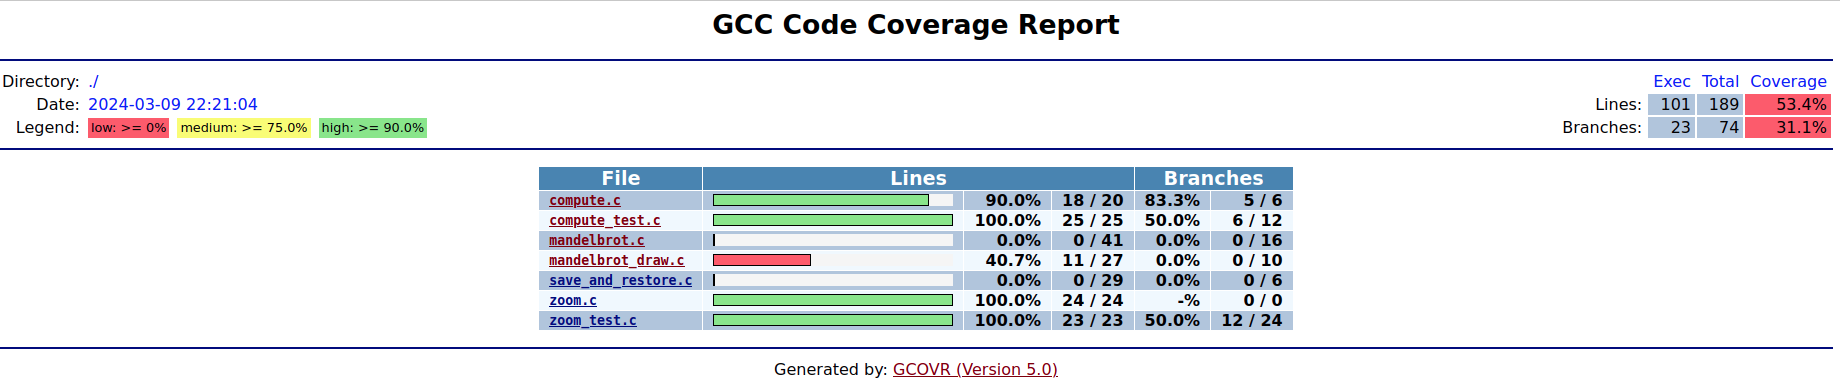
\includegraphics[width=1.0\linewidth]{Test-coverage}
	\caption[Test-coverage]{Screenshot der HTML-Ausgabe}
	\label{fig:Test-coverage}
\end{figure}
\end{sloppypar}

\section{Fazit}
Meiner Meinung nach besteht das Hauptziel dieses Projekts darin, die in diesem Semester erworbenen Kenntnisse der Programmiersprache C zu überprüfen. Außerdem ist das Mandelbrot-Projekt ein wunderbares Projekt, bei dem man die Kenntnisse der Mathematik anwenden muss. Dann muss man das ganze System mit den Kenntnissen der Programmierung realisieren. Nun kann das Programm nicht nur eine Konfiguration in einem bestimmten Ausschnitt grafisch darstellen, sondern auch in die Mandelbrotmenge hinein- und herauszoomen, eine Konfiguration speichern und laden, wenn bestimmte Tasten gedrückt werden. Und das Programm erfüllte alle fünf Anforderungen zu diesem Thema.  Ein weiterer erwähnenswerter Punkt bei diesem Projekt ist, dass dieses Programm auf verschiedenen Betriebssystemen laufen soll. Daher habe ich mein Makefile bereits so angepasst, dass mein Programm auf beiden Betriebssystemen, nämlich Ubuntu und MacOS, laufen kann.
\section{Verzeichnissse der Abbildungen und Listings}
\listoffigures
\listoflistings

\end{document}